

\begin{figure}[!tbp]
\begin{center}
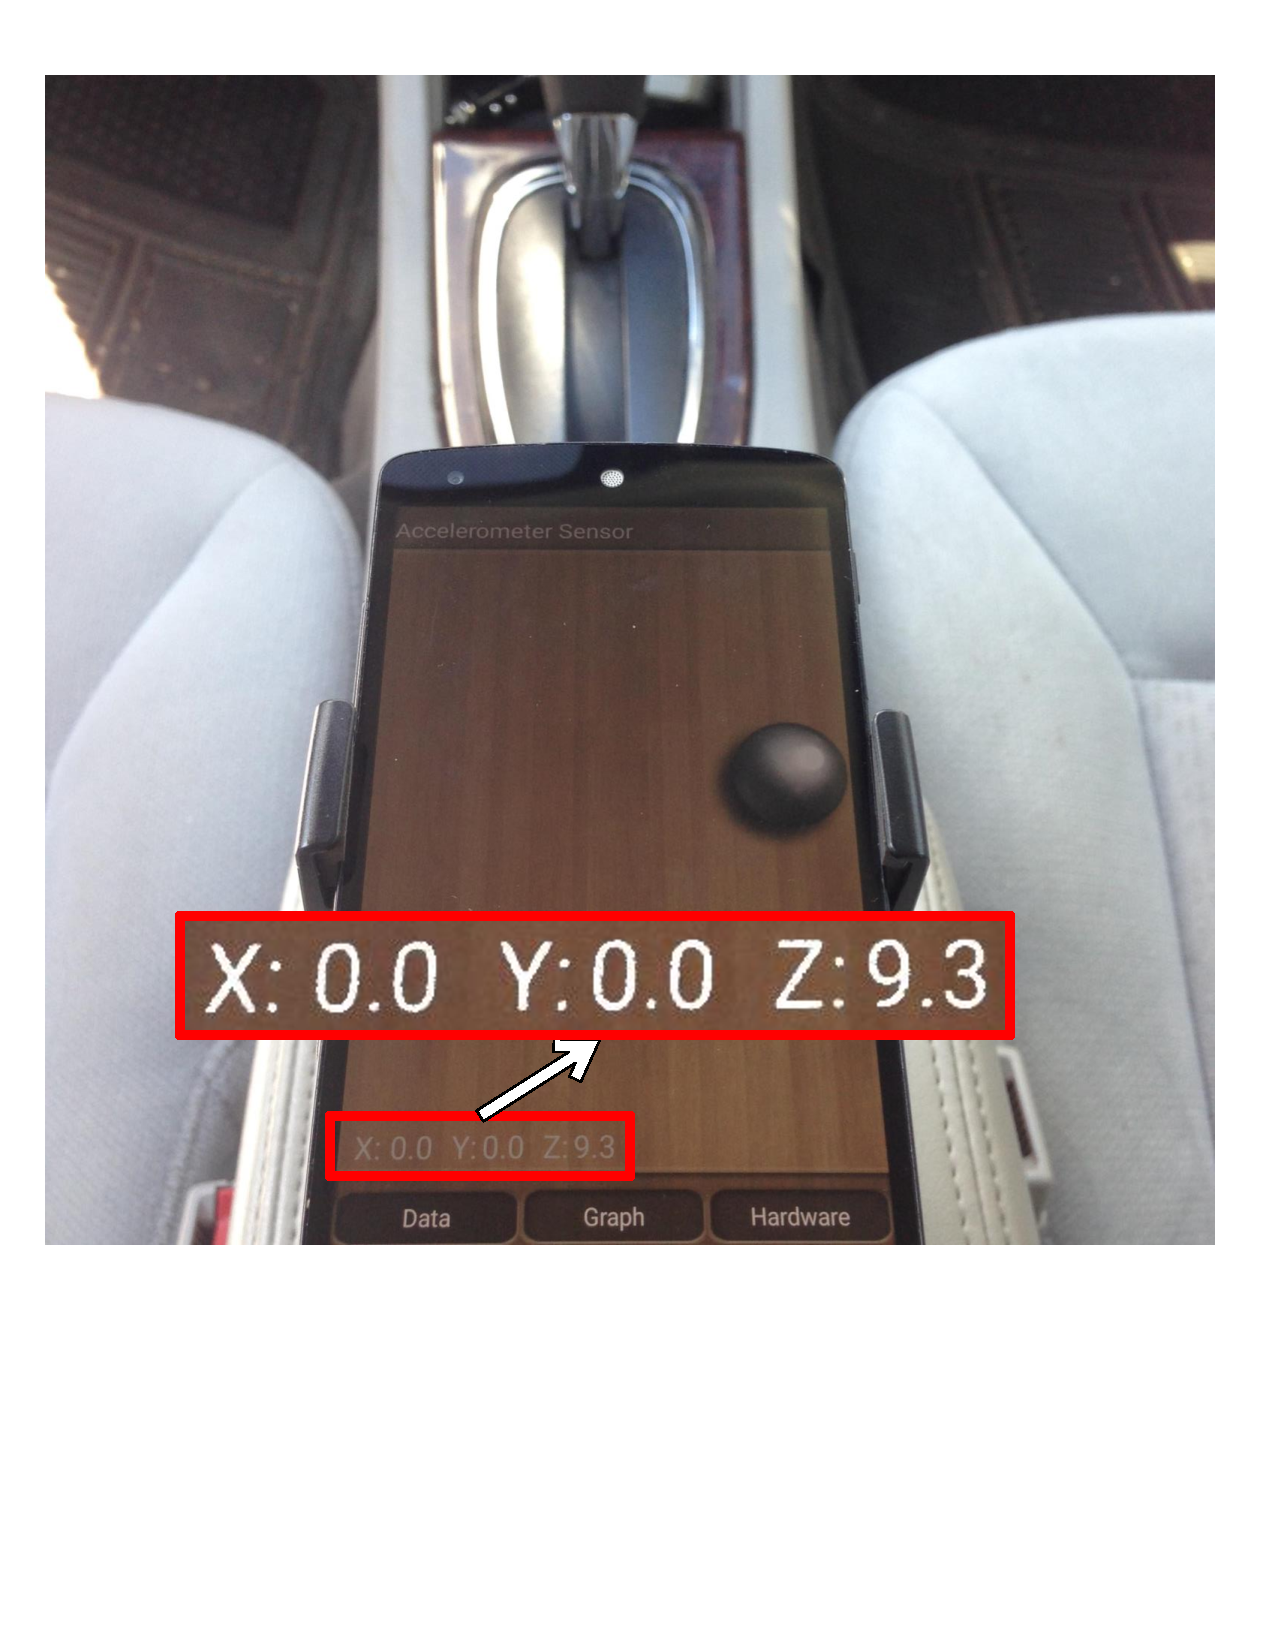
\includegraphics[width=2.0in, angle=0]{Figs/SlopeAware/placement.pdf}
\vspace{-1.5cm}
\caption{Manually aligned smartphone for the motivation example. 
The accelerometer readings are $[0.0, 0.0, 9.3]$.
Drivers usually mount their phones in arbitrary orientations.}
\vspace{-0.8cm}
\label{placement}
\end{center}
\end{figure}


In this section, we illustrate how road gradients can cause 
vehicle motion parameters overestimation or underestimation, 
which leads to false negatives/positives
when capturing driving behaviors such as brakes and accelerations.


\subsection{Motivation Experiment Setup}

We collected an example driving trip with various driving activities 
such as brakes and accelerations using a smartphone (LG Nexus 5).
Before the trip, we parked the car in a flat parking lot and fixed
the smartphone with a frame mounted between the driver seat
and the passenger seat.
As illustrated in Fig. \ref{placement}, the screen of the smartphone points to 
the sky and the y-axis is aligned with 
the car's heading direction.
The coordinates of the phone are manually aligned (as precisely as we can) with the car. 
It is impossible to perfectly align the coordinates 
manually or programmatically,
but we will show that the misalignment caused by manual placement
does not impact our observations.
The accelerometer reading in Fig. \ref{placement} is from a popular 
Android application called ``Android Sensor Box'' with one million downloads.
We used a customized Android application to record the sensor data and OBD speed data.
The sensor and OBD data traces of the trip are illustrated in Fig. \ref{motivation}.


\iffalse
\begin{figure}[!tbp]
\begin{center}
\subcaptionbox{\label{motivation_a}}{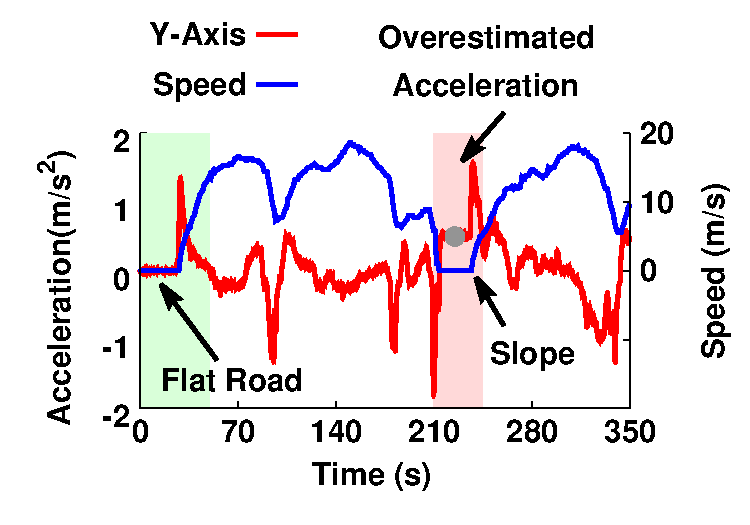
\includegraphics[width=3.3in,angle=0]{Figs/SlopeAware/motivation.pdf}}
\vspace*{-0.5cm}
%\setlength{\belowcaptionskip}{-3cm}
\subcaptionbox{\label{motivation_b}}{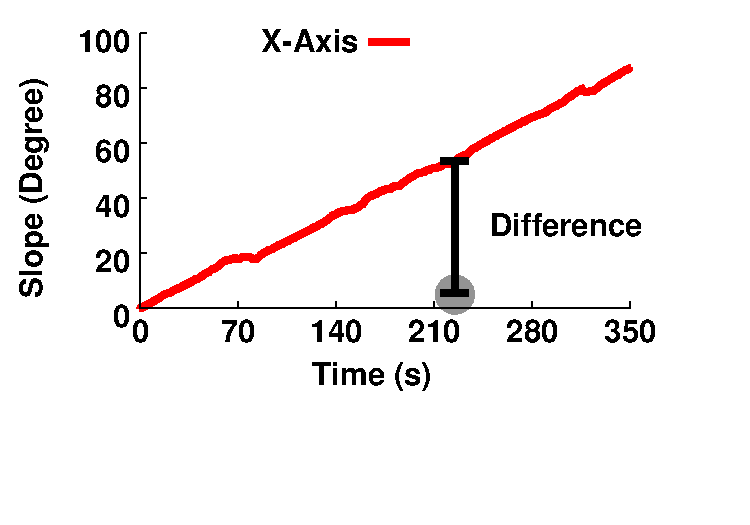
\includegraphics[width=3.3in,angle=0]{Figs/SlopeAware/gyro_motivation.pdf}}
\vspace*{-1.0cm}
\caption{The accelerometer y-axis (along the car's heading direction) and OBD speed readings 
	are plotted in the top figure.
The accumulated gyroscope x-axis (monitor car's rotated angles when going upslope/downslope) readings are plotted in the bottom figure.}
\label{motivation}
\vspace{-0.2cm}
\end{center}
\end{figure}
\fi

\begin{figure}[!tbp] \centering
 \begin{center}
  \begin{subfigure}[b]{\linewidth}
    \begin{center}
    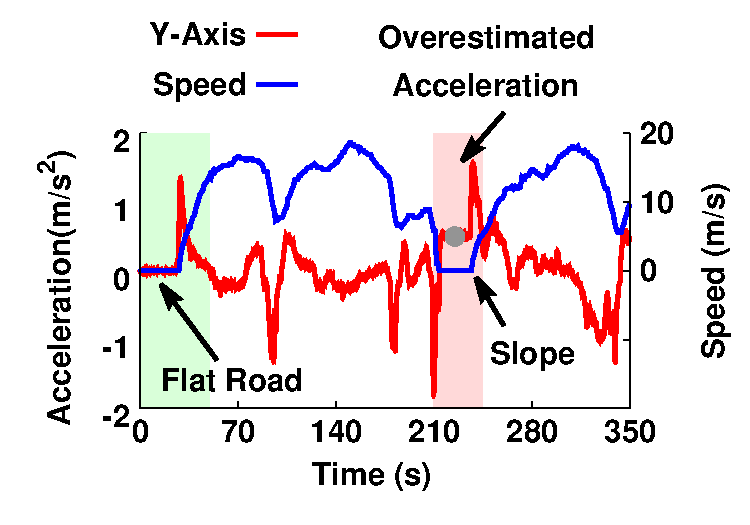
\includegraphics[width=3.3in,angle=0]{Figs/SlopeAware/motivation.pdf}
         \vspace{-0.4cm}
         \caption{The accelerometer y-axis (along the car's heading direction) and OBD speed readings.}         
        \label{motivation:a}
	\end{center}
    \end{subfigure} %

    \begin{subfigure}[b]{\linewidth}    
	    \begin{center}
        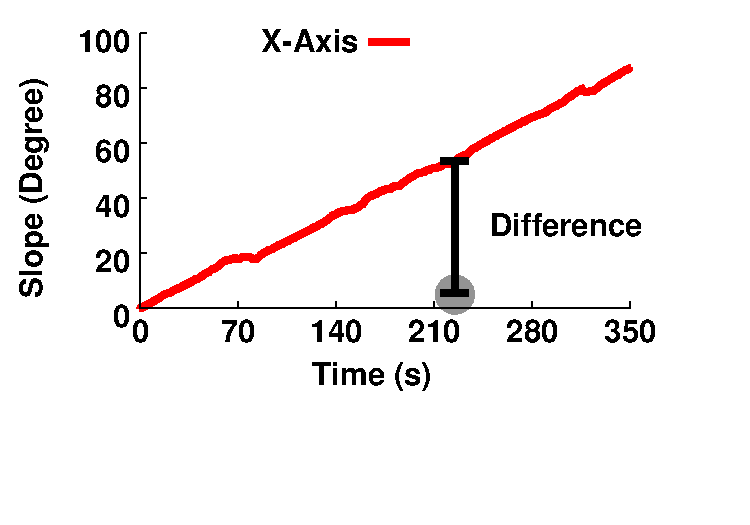
\includegraphics[width=3.3in,angle=0]{Figs/SlopeAware/gyro_motivation.pdf}
	\vspace{-1.5cm}
        \caption{The accumulated gyroscope x-axis (monitor car's rotational speed when going upslope/downslope) readings.}
        \label{motivation:b}
	 \end{center}
    \end{subfigure} 
\caption{Sensor and OBD data from the motivation example trip.}
\label{motivation}
\vspace{-0.2cm}
\end{center}
\end{figure}

\subsection{Acceleration Estimation Error}

As illustrated in Fig. \ref{motivation}, the trip started on a flat road
and the speed was $0m/s$ with acceleration $0m/s^2$. 
At time $210s$, there was a stop as the OBD speed reading was $0m/s$ 
while the accelerometer reading was around $0.5m/s^2$ indicating
the car was accelerating. It is an overestimated acceleration
due to road slope.
This is because the y-axis of the accelerometer can sense the gravity. 
The gravitational force may have an incremental or decremental effect
on the estimation of vehicle motion parameters. 
For example, a misalignment of five degrees may cause $0.85m/s^2$ 
acceleration estimation error.
For reference, the \emph{Snapshot Program} \cite{snapshot} records a hard brake if the deceleration is around $3m/s^2$.
Therefore, we conclude that \emph{road slopes and associated gravitational effect
cause acceleration overestimation or underestimation}. 


\begin{table}[!htbp]
\centering
    \caption[gravity]{Accelerometer Variance}
   \vspace{0.1cm}
    \label{gravity}
               \begin{tabular}{|l|c|}
 \hline
 Device & Gravity Reading ($m/s^2$) 
 \\  \hline      \hline
LG Nexus 5 & 9.33       
 \\  \hline
Galaxy SII & 9.61
 \\   \hline
Nexus 9 & 9.78
 \\  \hline
Nexus 5x & 10.01
 \\  \hline
 \end{tabular}
\end{table}


Another source of acceleration estimation error comes from \emph{device variance}.
Different accelerometers in different smartphones have different sensitivities.
For example, different accelerometers have different gravity readings at steady state, where the gravity force is known to be about $9.8m/s^2$.
We summarize the gravity reading of different devices/accelerometers 
in Table \ref{gravity}.
The accelerometer reading differences among different devices can be up to $0.75m/s^2$.


To capture the real acceleration of a car, we are interested in the
\emph{linear acceleration} along the car's moving directions.
There is an estimated linear acceleration sensor type in the
Android sensor event implementation \cite{androidsourcecode}. 
But it is derived from the accelerometer minus the gravitational components along each dimension,
and its accuracy highly relies on the orientation estimation.
The default orientation estimation implementation of Android is known to be inaccurate \cite{zhou2014use}.
Therefore, it is unable to be used in vehicular settings. 


\subsection{Accumulated Gyroscope Errors}

The gyroscope can be used to track three-dimensional angular changes
and is an ideal input for slope estimation. 
However, it is known to suffer accumulated errors \cite{zhou2014use}. 
As illustrate in Fig. \ref{motivation}, 
we observe similar error accumulation in our motivation experiment. 
The dark dot is the slope gradient calculated by the accelerometer.
The curve of gyroscope measures the accumulated angular changes  
when the car was driving upslope/downslope.
Intuitively, the accumulated angular change of gyroscope can be used to 
estimate the slope gradients.
Clearly, the accumulated error is much higher than 
the actual accumulated slope gradients estimated by the accelerometer. 
We refer interested readers to \cite{chen2015invisible, zhou2014use},  
for detailed gyroscope three-dimensional readings 
and corresponding vehicle movement. 
Since we only focus on going upslope/downslope, we are interested in 
x-axis gyroscope readings of the car (or aligned smartphone) only.

There are several reasons why we see accumulated errors of gyroscope. 
The first one is the constant drifts, where the gyroscope reading is 
not zero in still due to limited hardware precision.
As the angular changes add up, the constant drifts accumulate correspondingly, 
which leads to a rough linear function between accumulated error and time.
The second one is the vibration of the vehicle, which accelerates
the drifts of the gyroscope readings.
Misalignment (caused by either manual alignment in our experiment 
or the coordinate alignment algorithm) between the car and the smartphone can also introduce accumulated errors. 
This is because the x-axis of the gyroscope can also sense car's steering angular change like turns and lane changes
when the smartphone is misaligned with the car.

\subsection{Road Slope Statistics}

\iffalse
\begin{figure}[!htbp]
\begin{center}
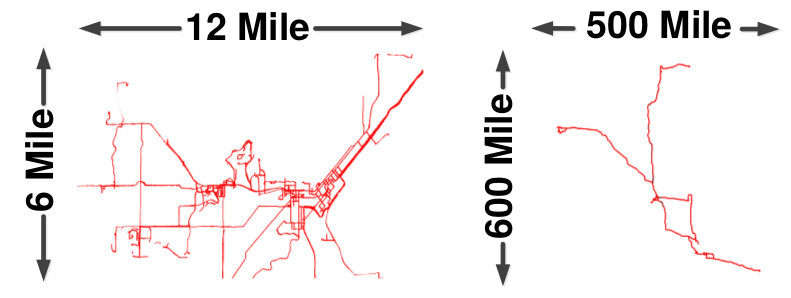
\includegraphics[width=3.2in, angle=0]{Figs/SlopeAware/urbanhighwaymap.png}
\vspace{-0.0cm}
\caption{Urban driving data (left) are collected from a US mid-size city.  
Highway driving data (right) are collected from both local highways and cross-state highways. 
The maps are removed for the double-blind review.}
\vspace{-0.3cm}
\label{coverage}
\end{center}
\end{figure}
\fi

\begin{figure}[!htbp]
\begin{center}
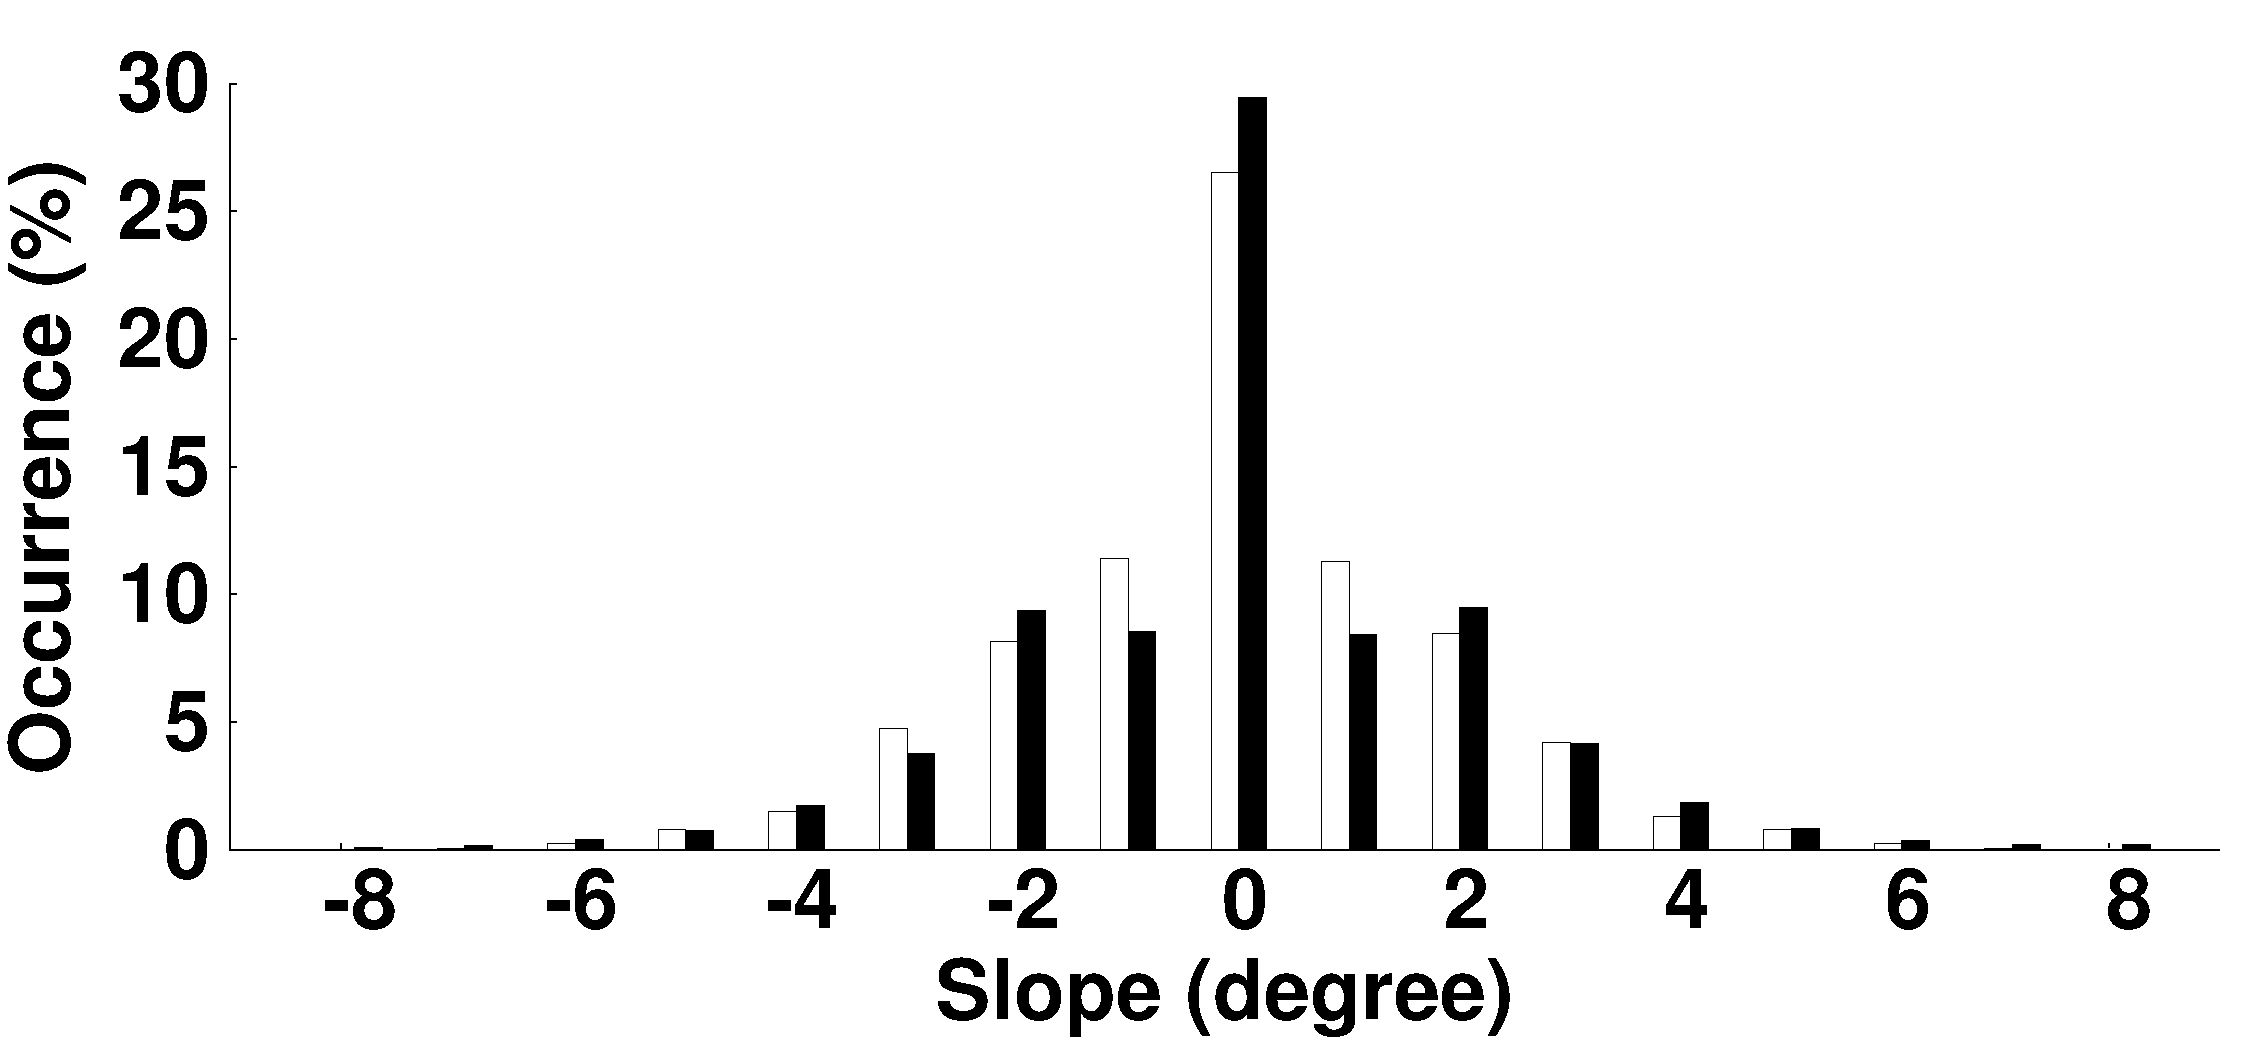
\includegraphics[width=3.3in,angle=0]{Figs/SlopeAware/degrees.pdf}
\vspace{0.0cm}
\caption{Histogram of slope gradients.}
\label{slopegradients}
\vspace{-0.4cm}
\end{center}
\end{figure}



As we discussed above, the slopes introduce linear acceleration estimation errors.
An important question is how many road segments are sloping and
how many of them are actually level. 
Some cities, e.g., San Diego and Los Angeles, are full of hills, 
and most roads are sloping roads.
Surprisingly, in the plain area of the northwestern US, 
there are also full of slopes. 
We collected a dataset that contains sensor data, GPS and OBD readings.
The dataset is collected from 13 drivers over the course of two years. 
The map coverage of the dataset is shown in Fig. \ref{rpm_gph}. 
The dataset consists of urban data from a US mid-size city and highway data 
that from five different states in the northwestern US.


To obtain the road gradient, we use the Google elevation dataset \cite{googleelevation}. 
For each GPS data point, we queried the elevation from the dataset. 
and calculated the gradient by the elevation difference
and distance.
We eliminated the close consecutive GPS data points that less than 5 meters in distance and removed the data points where the speed is less than $10mph$.
As we can see from the histogram in Fig. \ref{slopegradients}, 
more than half of the roads are not flat.
Those sloping roads, even as small as two degrees, may introduce accumulated
errors on coordinate alignment and further slope estimation.
The aggregated error may cause significant linear acceleration estimation error
and introduce false positives/negatives on brake/acceleration monitoring. 






%%%%%%%%%%%%%%%%%%%%%%%%%%%%%%%The End%%%%%%%%%%%%%%%%%%%%%%%%%%%%%%%%%%%%%%%

\iffalse
\begin{figure}[h]
\begin{center}
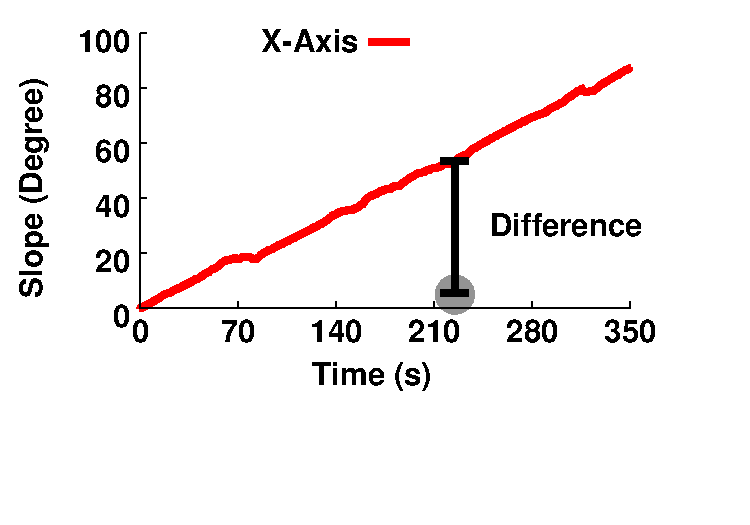
\includegraphics[width=3.3in,angle=0]{Figs/SlopeAware/gyro_motivation.pdf}
\vspace{0.0cm}
\caption{Gyroscope drift.}
\label{gyrodrift}
\vspace{-0.2cm}
\end{center}
\end{figure}
\fi

\iffalse
\begin{figure}[h]
\begin{center}
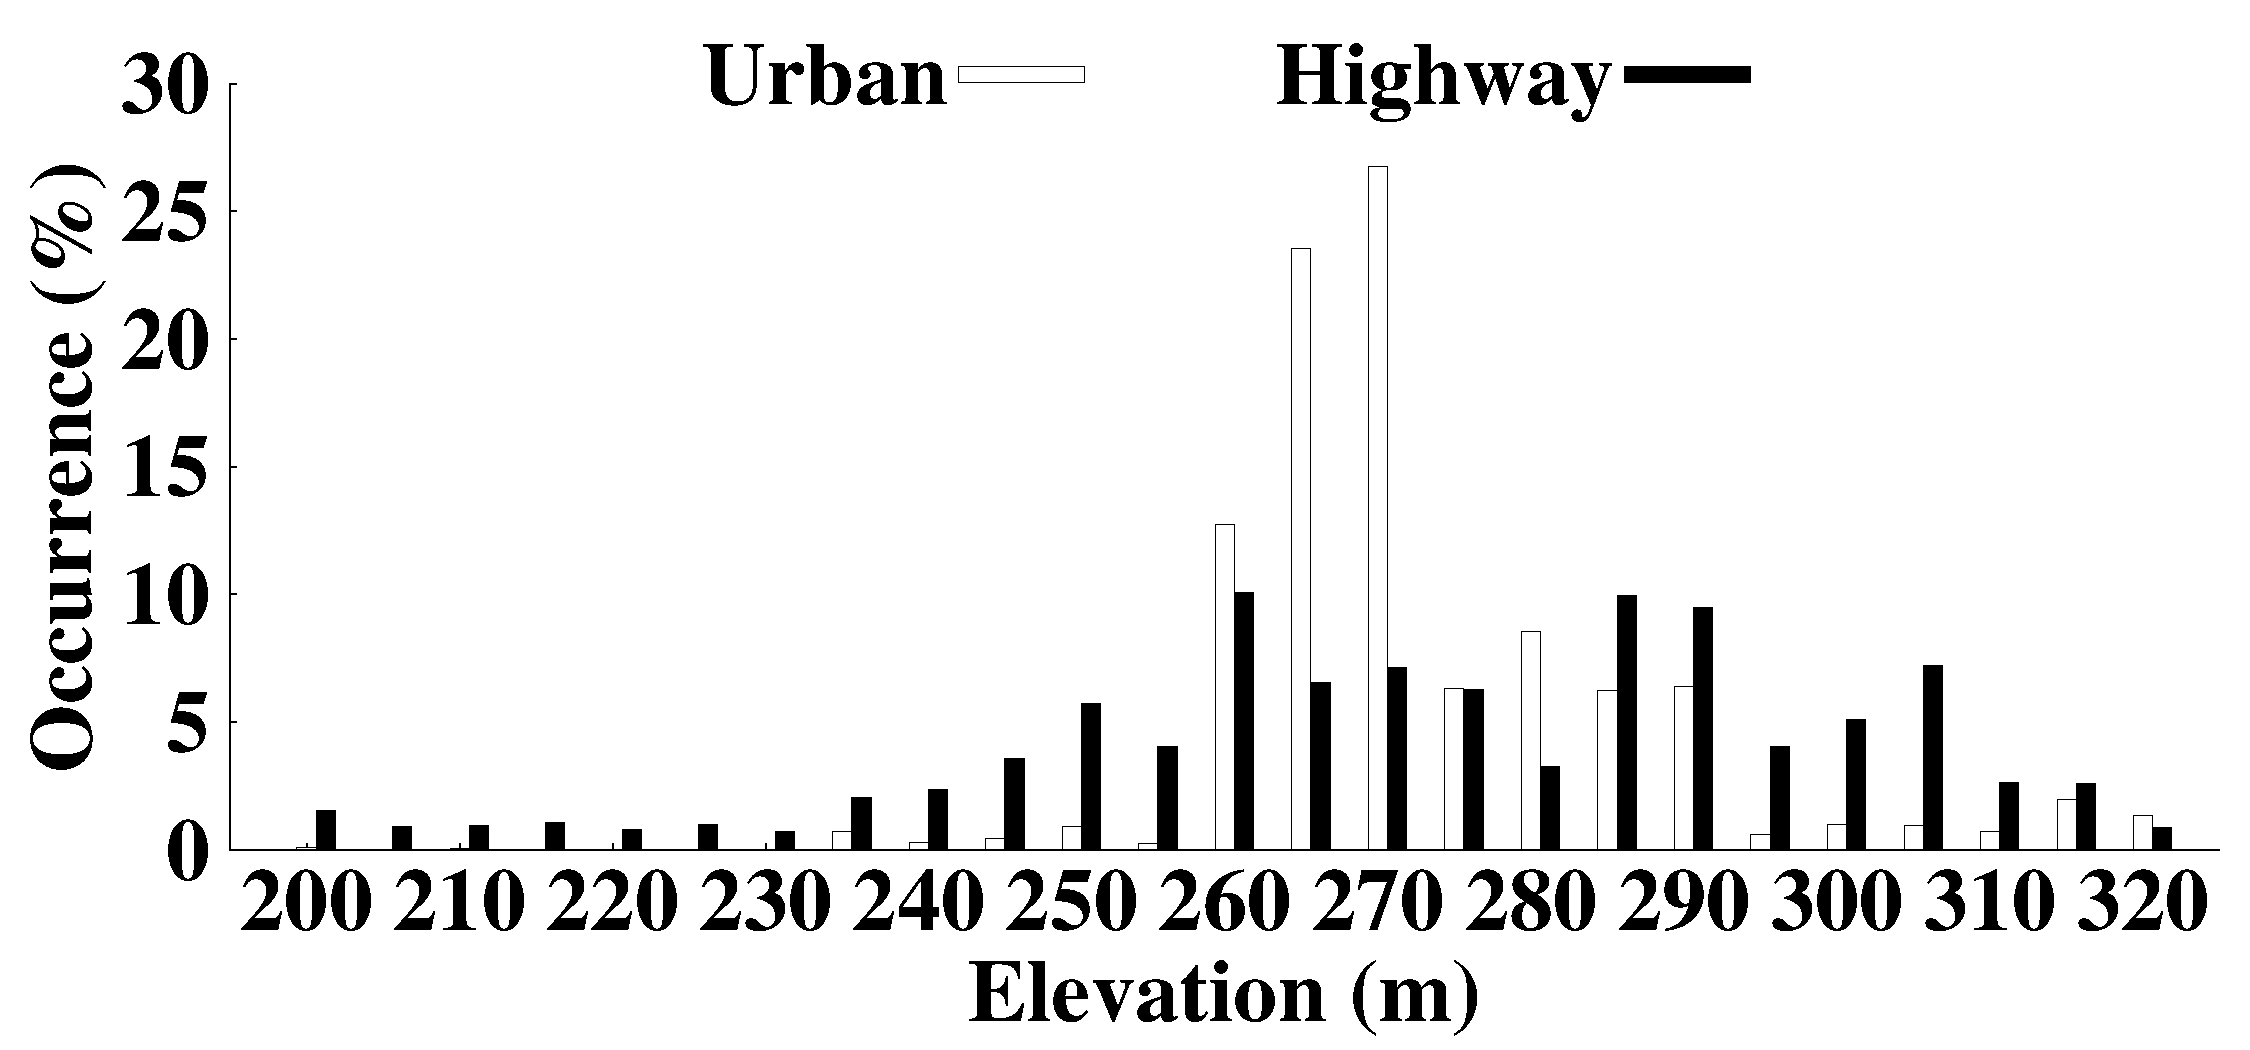
\includegraphics[width=3.3in,angle=0]{Figs/SlopeAware/elevation.pdf}
\vspace{0.0cm}
\caption{Elevation comparison of data collected from urban and highway roads.}
\label{elevation}
\vspace{-0.2cm}
\end{center}
\end{figure}
\fi


